\section{Teste de localização com smartphone}
\label{sec:teste-smarphone}

Para verificar a capacidade dos sensores de localizar contextualmente um
dispositivo móvel, um \emph{smartphone} foi utilizado. Este foi posicionado em duas salas
diferentes, sendo que em cada uma delas foi executada uma captura de 10 minutos. Para
que houvesse tráfego na rede, o dispositivo móvel foi configurado para receber um
\emph{stream} de vídeo no aplicativo \emph{Netflix}.

\begin{figure}[htb]
	\caption{\label{fig-planta-baixa}Ambiente de teste}
	\begin{center}
		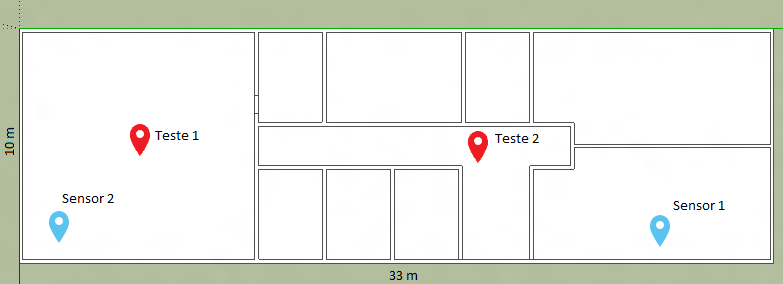
\includegraphics[width=1\textwidth]{060-testes/data-analisis/planta-baixa-smartphone.png}
	\end{center}
	\nota[Em azul]{Sensores da aplicação}%
	\nota[Em vermelho]{Pontos do dispositivo teste}%
	\legend{Fonte: Elaborada pelo autor}
\end{figure}


No teste 1, o dispositivo estava na mesma sala do sensor 2. As distâncias
aproximadas, em linha reta, entre o ponto teste 1 e o sensor 1 é de \texttt{21,52m} e
entre o mesmo ponto e o sensor 2 é de \texttt{7,00m}. Foram capturados
\texttt{157.736} pacotes, totalizando \texttt{9,7 MB} pelo sensor 1 e \texttt{21.
974} pacotes, totalizando \texttt{1.9 MB} de captura pelo sensor 2.

Para o teste 2, o dispositivo móvel estava posicionado no corredor fora da sala
do sensor 1 e distante do sensor 2. As distâncias aproximadas, em linha reta, entre o
ponto de teste 2 e o sensor 1 é de \texttt{9,35m} e entre o mesmo ponto e o sensor
2 é de \texttt{20,14m}. Neste teste, o sensor 1 capturou \texttt{103.555} pacotes,
totalizando \texttt{6.4 MB} de captura. Já o sensor 2 capturou \texttt{22.635}
pacotes totalizando \texttt{2 MB} de captura.

Posteriormente, os arquivos de captura foram analisados com a ferramenta
\emph{Ron’s Editor} para que o \texttt{``summary''} fosse construído.

\clearpage
\begin{figure}[ht]
	\centering
	\caption{\label{fig-mg4-noise-t1}Sumário de pacotes por dispositivo - Teste 1}
	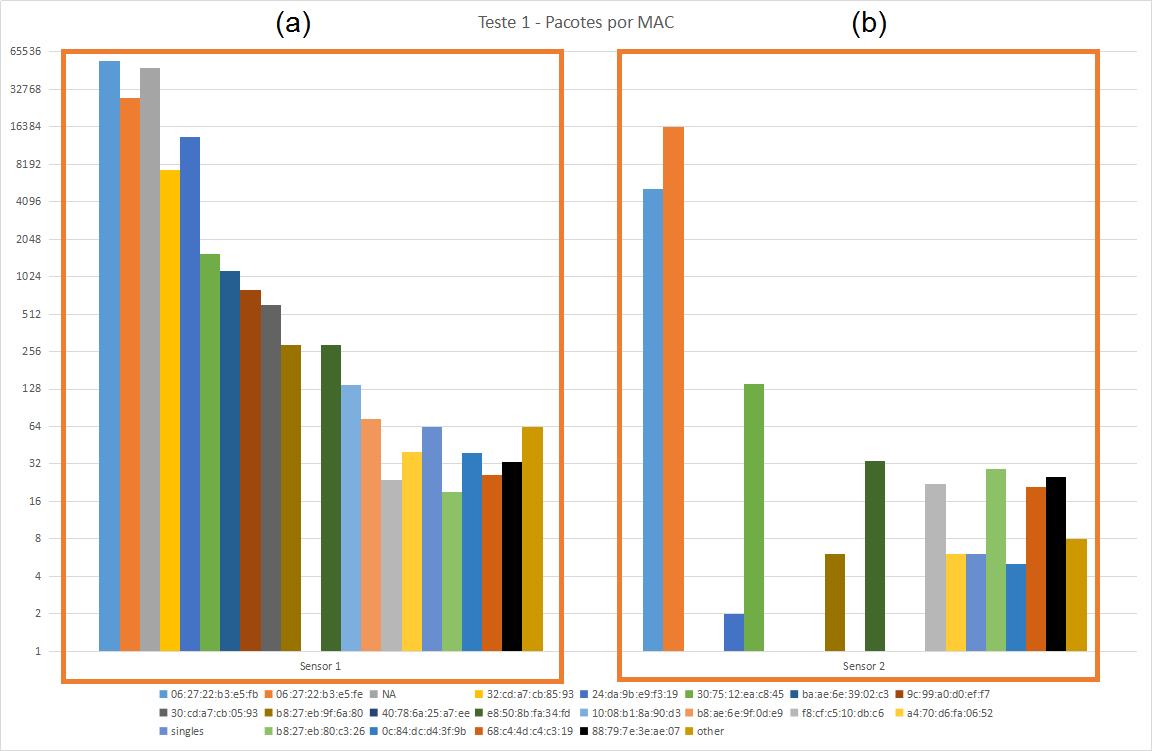
\includegraphics[height=0.32\textheight,width=1\textwidth]{060-testes/data-analisis/distance-mg4plus-netflix/Teste1.png}
	\legend{À esquerda, os pacotes recebidos pelo sensor 1 e a direita do sensor 2.
	Em preto, o dispositivo móvel. Fonte: Elaborada pelo autor}
\end{figure}

\begin{figure}[hb]
	\centering
	\caption{\label{fig-mg4-noise-t2}Sumário de pacotes por dispositivo - Teste 2}
	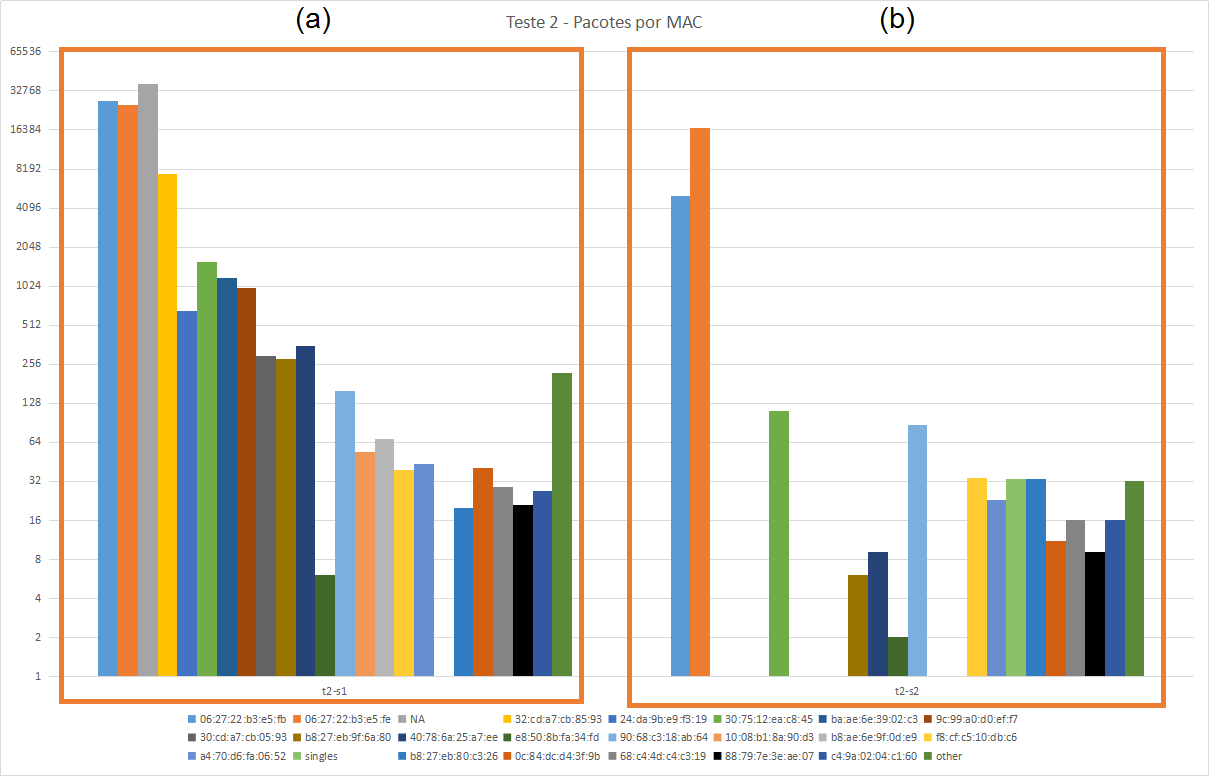
\includegraphics[height=0.32\textheight,width=1\textwidth]{060-testes/data-analisis/distance-mg4plus-netflix/Teste2.png}
	\legend{À esquerda, os pacotes recebidos pelo sensor 1 e a direita do sensor 2.
	Em preto, o dispositivo móvel.
	Fonte: Elaborada pelo autor.}
\end{figure}

Pode-se observar que o \emph{smartphone} não representa a maioria dos pacotes
capturados, evidenciando a constatação do ambiente real e ruidoso em que o teste foi
executado.

\clearpage

Entretanto, uma vez filtrado os pacotes onde o endereço MAC do transmissor é o do
\emph{smartphone}, pode-se inferir os valores médios de potência de sinal o desvio padrão, chegando
nos seguinte valores.

\begin{table}[htb]
\IBGEtab{%
\ABNTEXchapterfont {
	\caption{\label{table:smartphone-distance}Análise dos pacotes do \emph{smartphone} - 10 minutos}%
}
}{%
\begin{tabular}{c|cc|cc}
\toprule
\midrule
Teste							& \multicolumn{2}{c|}{teste 1}			&	\multicolumn{2}{c}{teste 2}	\\
\midrule
Sensor 							&	Sensor 1		&	Sensor 2		&	Sensor 1		&	Sensor 2	\\
\midrule
Pacotes							&	33				&	25				&	21				&	9			\\
$\overline{dBm}$				&	-76.6969697		&	-49.88			&	-53.95238095	&	-68.55555556\\
$\sigma$						&	2.833778931		&	2.833137248		&	4.177034719		&	3.431876714	\\
\midrule
\midrule
$d(\overline{dBm})$				&	68.36730882		&	3.118889584		&	4.984470702		&	26.77797784	\\
$d(\overline{dBm} - \sigma)$	&	49.33550049		&	2.250832294		&	3.081536468		&	18.03781557	\\
$d(\overline{dBm} + \sigma)$	&	94.74088372		&	4.321722353		&	8.062519603		&	39.75315605	\\
Erro acumulado metros			&	45.40538323		&	2.070890059		&	4.980983136		&	21.71534048	\\
\midrule
\midrule
Distância real $M$				&	21.52			&	7				&	9.35			&	20.14		\\
$d(\overline{dBm}) - M$			&	46.84730882		&	3.881110416		&	4.365529298		&	6.637977837	\\
\midrule
\bottomrule
\end{tabular}%
}{%
	\fonte{Produzido pelo autor.}%
}
\end{table}

Os mesmos padrões encontrados na \autoref{sec:teste-ruido} aparecem: desvio
padrão grande e erro acumulado maior ainda. Porém, este trabalho limita-se a determinar o contexto (sala, área, etc.), sendo que esta resposta pode
ser vista no contraste das \autoref{fig-mg4-t1} e \autoref{fig-mg4-t2} onde a
mudança do contexto é mais clara. Nestas figuras, plota-se em gráficos
as médias encontradas na \autoref{table:smartphone-distance}.

No teste 1, na figura \autoref{fig-mg4-t1}, a potência de sinal (RSS) do dispositivo é maior em relação ao
\texttt{sensor 2} ($-49,88$ é maior que $-76,70$). Portanto, pode-se inferir que o
dispositivo móvel estava mais inserido no contexto do \texttt{sensor 2} do que no contexto
do \texttt{sensor 1}, o que se confirma no ambiente físico.

No teste 2, na figura \autoref{fig-mg4-t2}, o dispositivo obteve uma potência de sinal maior em relação ao
\texttt{sensor 1} ($-53,95$ é maior que $-68,56$), ou seja, estava mais inserido no contexto
do \texttt{sensor 1}, o que também se confirma no ambiente de teste.

A partir dos resultados acima, pode-se concluir que os sensores não possuem
precisão quanto à distância geográfica que o dispositivo móvel se encontra de
cada sensor, mas há um certa precisão quanto ao contexto. Então, é possível
dizer em que contexto o \emph{smartphone} estava inserido. Portanto,
a potência não revela-se útil para o posicionamento de geolocalização
(coordenadas e distâncias), mas sim para uma localização
contextual em que associa-se um dispositivo ao contexto do sensor.


\begin{figure}[htb]
	\label{mg4-distance}
	\centering
	\begin{minipage}{0.49\textwidth}
	\centering
		\caption{\label{fig-mg4-t1}dBm Motorola G4+ - Teste 1}
		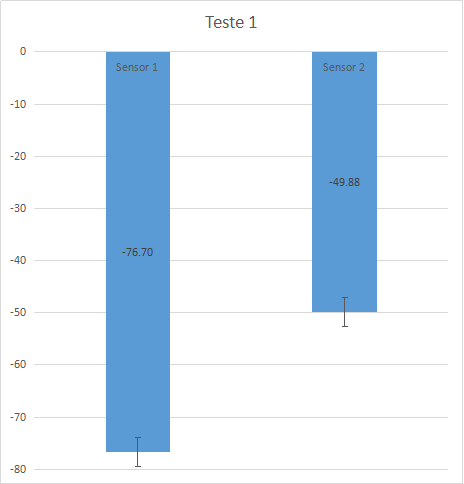
\includegraphics[width=1\textwidth]{060-testes/data-analisis/distance-mg4plus-netflix/target-Teste1.png}
		\legend{Fonte: Elaborada pelo autor}
	\end{minipage}
	\hfill
	\begin{minipage}{0.49\textwidth}
	\centering
		\caption{\label{fig-mg4-t2}dBm Motorola G4+ - Teste 2}
		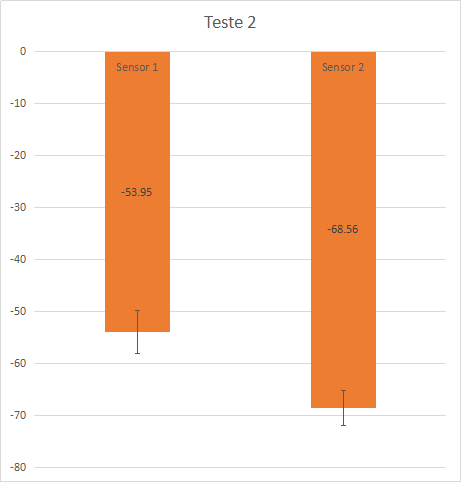
\includegraphics[width=1\textwidth]{060-testes/data-analisis/distance-mg4plus-netflix/target-Teste2.png}
		\legend{Fonte: Elaborada pelo autor}
	\end{minipage}
\end{figure}
